\chapter*{\textsc{Introduction}}
\addcontentsline{toc}{chapter}{\textsc{Introduction}}
	
	\paragraph{Objectifs}
	\begin{itemize} [label=\ding{70},font=\small \color{black}]
	\item Développer une commande pour la fonction de contrôle et d’évacuation de la maquette de Banc de Contrôle Industriel (BCI).
	\item Mettre en pratique la démarche systématique de modélisation vue lors du cours et des TD.
	\end{itemize}
	
	\paragraph{Système de commande\\}

	La fonction de contôle et d'évacuation de la maquette de BCI permet de trier deux types de pièces arrivant de manière désordonnée sur un convoyeur à tapis roulant $(A5)$. Voici les pièces que nous considérerons:  
	\begin{itemize} [label=\ding{171},font=\small \color{black}]
	\item Les pièces hautes grises, embases métalliques que l'on assimilera à des bouteilles.
	\item Les pièces basses blaches, anneaux en matière plastique que l'on assimilera à des bouchons.
	\item On appelera assemblage lorsqu'un anneau est emboîté sur une embase.\\ 
	\end{itemize}
	
	Les capteurs et actionneurs qui sont liés à cette fonction sont les suivants :
	\begin{itemize} [label=\ding{70},font=\small \color{black}]
	\item $A3 :$ actionneur linéaire à solénoïde, permet d’éjecter une pièce de la zone d’éjection.
	\item $A5 :$ moteur du convoyeur à bande (tapis roulant) apportant des pièces vers la zone de contrôle et la zone d’éjection.
	\item $C4 :$ détecteur photo-électrique par barrage, détecte toutes les pièces arrivant vers la zone de contrôle.
	\item $C5 :$ détecteur photo-électrique de proximité, détecte toutes les pièces dans la zone de contrôle.
	\item $C6 :$ détecteur photo-électrique de proximité, détecte toutes les pièces dans la zone d'éjection.
	\item $C7 :$ détecteur de proximité inductif, détecte les bouteilles et les assemblages, arrivant vers la zone de contrôle.
	\item $C8 :$ détecteur de proximité capacitif placé en hauteur, détecte les pièces hautes (assemblages) dans la zone de contrôle.
	\end{itemize}
	
	\begin{center}
	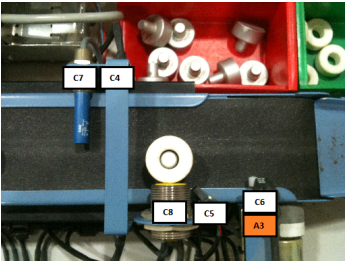
\includegraphics[scale=0.75]{zone.png}
	\captionof{figure}{\textit{zones de contrôle et d'éjection du BCI}}
	\label{fig1}
	\end{center}  

	\paragraph{Travail à réaliser\\}
		Posons les hypothèses suivants:
		\begin{itemize} [label=\ding{70},font=\small \color{black}]
		\item Au maximum une pièce est présente entre les capteurs $C7$ et $C6$.
		\item Le convoyeur à bande $A5$ sera supposé actif à tout instant.
		\end{itemize}